%==============================================================================
% Sjabloon poster bachproef
%==============================================================================
% Gebaseerd op document class `a0poster' door Gerlinde Kettl en Matthias Weiser
% Aangepast voor gebruik aan HOGENT door Jens Buysse en Bert Van Vreckem

\documentclass[a0,portrait]{hogent-poster}

% Info over de opleiding
\course{Bachelorproef}
\studyprogramme{toegepaste informatica}
\academicyear{2024-2025}
\institution{Hogeschool Gent, Valentin Vaerwyckweg 1, 9000 Gent}

% Info over de bachelorproef
\title{Real-time vertaling van Vlaamse Gebarentaal naar tekst op een mobiel apparaat.}
\subtitle{Ondertitel (eventueel)}
\author{Tom Deganck}
\email{tom.deganck@student.hogent.be}
\supervisor{Stijn Lievens}
\cosupervisor{Kim Van Mele}

% Indien ingevuld, wordt deze informatie toegevoegd aan het einde van de
% abstract. Zet in commentaar als je dit niet wilt.
\specialisation{AI \& Data Engineer}
\keywords{Sign Language, Computer Vision, Machine Learning, Deep Learning, Convolutional Neural Networks}
\projectrepo{https://github.com/TomDeganck/latex-hogent-bachproef-main}

\begin{document}

\maketitle

\begin{abstract}
Inclusieve communicatie is essentieel.
Dit onderzoek verkent hoe real-time vertaling van Vlaamse Gebarentaal (VGT) naar tekst via computer vision de kloof verkleint tussen doven, slechthorenden, mensen met spraak-/taalstoornissen en de horende samenleving. 
Bestaande hulpmiddelen zijn vaak niet snel of toegankelijk genoeg.
\end{abstract}

\begin{multicols}{2} % This is how many columns your poster will be broken into, a portrait poster is generally split into 2 columns

\section{Introductie}

Technologische vooruitgang, met name op het gebied van deep learning, biedt ongekende kansen om de communicatie tussen doven en horenden te verbeteren. 
Dit onderzoek duikt in de toepassing van bestaande pre-getrainde deep learning-modellen voor real-time gebarentaalherkenning. 
Onze focus ligt op de implementatie van een mobiele applicatie, waarbij we de afwegingen tussen on-device en cloud-gebaseerde implementatie onderzoeken om de beste balans te vinden tussen latentie, prestaties en toegankelijkheid. 
Kom meer te weten over onze methodologie en de implicaties voor de toekomst van gebarentaaltechnologie.

\section{Experimenten}


\section{Sectie met figuur}

De {\LaTeX} figure-omgeving bepaalt zelf waar een afbeelding komt en dat is meestal niet op de plek in de tekst waar de figure-omgeving gedefinieerd wordt. Als je wilt forceren dat afbeeldingen toch in de flow van de tekst blijven, dan kan je dat zoals hieronder:

\begin{center}
  \captionsetup{type=figure}
  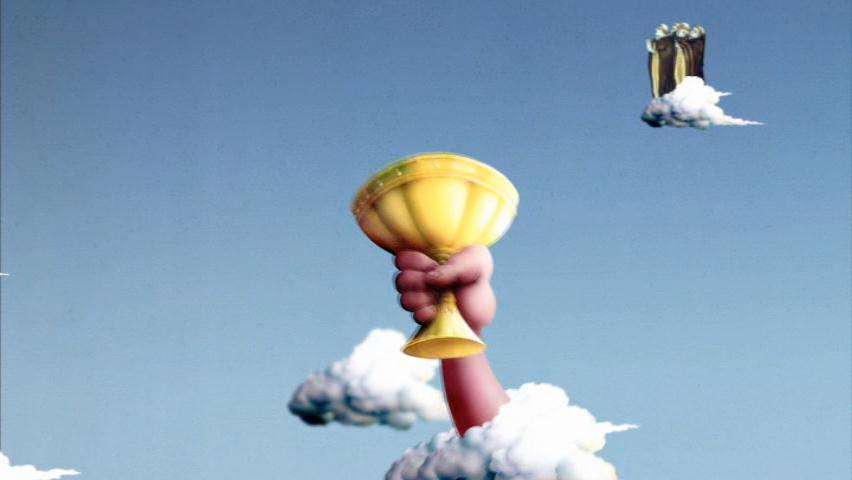
\includegraphics[width=1.0\linewidth]{grail}
  \captionof{figure}{He hasn't got shit all over him. The nose? Where'd you get the coconuts? What do you mean? We shall say `Ni' again to you, if you do not appease us}
\end{center}

Let er wel op dat dit tot problemen met bladschikking kan leiden.

\section{Conclusies}

Don't underestimate the Force. Oh God, my uncle. How am I ever gonna explain this? I suggest you try it again, Luke. This time, let go your conscious self and act on instinct. Don't be too proud of this technological terror you've constructed. The ability to destroy a planet is insignificant next to the power of the Force.

\section{Toekomstig onderzoek}

I care. So, what do you think of her, Han? No! Alderaan is peaceful. We have no weapons. You can't possibly… I have traced the Rebel spies to her. Now she is my only link to finding their secret base.

Kid, I've flown from one side of this galaxy to the other. I've seen a lot of strange stuff, but I've never seen anything to make me believe there's one all-powerful Force controlling everything. There's no mystical energy field that controls my destiny. It's all a lot of simple tricks and nonsense. You are a part of the Rebel Alliance and a traitor! Take her away! 

\end{multicols}
\end{document}